% QCAA HW3 report -- compile with XeLaTeX (build_report.py)
% Numerical tables/macros in generated/ are produced by build_report.py
% from results/*.json; do not edit them by hand.
\documentclass[11pt,a4paper]{article}

\usepackage{amsmath,amssymb,bm}
\usepackage{geometry}
\geometry{margin=2.3cm}
\usepackage{graphicx}
\graphicspath{{../figures/}}
\usepackage{booktabs}
\usepackage{array}
\usepackage{float}
\usepackage{caption}
\usepackage{hyperref}
\hypersetup{colorlinks=true,linkcolor=blue!60!black,urlcolor=blue!60!black}
\usepackage{xcolor}

\newcommand{\Ha}{\,\mathrm{Ha}}
\newcommand{\ket}[1]{\lvert #1 \rangle}
\newcommand{\bra}[1]{\langle #1 \rvert}
\newcommand{\braket}[2]{\langle #1 \vert #2 \rangle}

\newcommand{\PkgVersions}{PennyLane 0.44.1, OpenFermion 1.7.1, Qiskit 2.3.0, NumPy 2.4.4}
\newcommand{\PLVersion}{0.44.1}
\newcommand{\Enuc}{+0.71375399}
\newcommand{\ErhfHtwo}{-1.11668}
\newcommand{\EfciHtwo}{-1.13727}
\newcommand{\EfciHtwoLong}{-1.13727017}
\newcommand{\ErhfLih}{-7.86200}
\newcommand{\EfciLih}{-7.88239}
\newcommand{\EfciLihLong}{-7.88239152}
\newcommand{\PoneHaa}{-1.83043838}
\newcommand{\PoneHab}{+0.18128881}
\newcommand{\PoneHbb}{-0.25450368}
\newcommand{\PoneHermDev}{\ensuremath{8.3\times10^{-17}}}
\newcommand{\PoneSqDev}{\ensuremath{0}}
\newcommand{\PoneCoupling}{\ensuremath{1.0\times10^{-16}}}
\newcommand{\PoneFciErr}{\ensuremath{1.7\times10^{-7}}}
\newcommand{\PoneCa}{-0.9936}
\newcommand{\PoneCb}{+0.1128}
\newcommand{\PoneCtwoSq}{0.0127}
\newcommand{\PoneEcorr}{-0.0206}
\newcommand{\PoneCorrLast}{0.278}
\newcommand{\PtwoAcrDev}{\ensuremath{1.0\times10^{-16}}}
\newcommand{\PtwoNumDev}{\ensuremath{1.0\times10^{-16}}}
\newcommand{\PtwoBeleven}{+0.04532220}
\newcommand{\PtwoSectorDev}{\ensuremath{3.7\times10^{-14}}}
\newcommand{\PtwoFciErr}{\ensuremath{1.7\times10^{-7}}}
\newcommand{\PthreePermDev}{\ensuremath{2.5\times10^{-16}}}
\newcommand{\PthreeBrillouin}{\ensuremath{1.0\times10^{-16}}}
\newcommand{\PthreeThetaOpt}{-0.113068}
\newcommand{\PthreeCxJw}{48}
\newcommand{\PthreeCxPar}{4}
\newcommand{\PfourTone}{232}
\newcommand{\PfourTtwo}{150}
\newcommand{\PfourSxErr}{\ensuremath{2.4\times10^{-4}}}
\newcommand{\PfourEcrErr}{\ensuremath{7.7\times10^{-3}}}
\newcommand{\PfourRoErr}{\ensuremath{2.0\times10^{-2}}}
\newcommand{\PfourNoisyBias}{0.073}
\newcommand{\PfiveSectorProb}{1.000000000000}
\newcommand{\PfiveEnuc}{+0.99488}
\newcommand{\PfiveCcsdIter}{52}
\newcommand{\PfiveEccsd}{-7.88238102}
\newcommand{\PfiveCcsdErr}{\ensuremath{1.0\times10^{-6}}}
\newcommand{\PfiveEucc}{-7.88237783}
\newcommand{\PfiveUccErr}{\ensuremath{1.4\times10^{-5}}}
\newcommand{\PfiveFinalErr}{\ensuremath{8.4\times10^{-5}}}


\title{Quantum Computing Algorithms and Applications\\Homework 3}
\author{Student ID: B13705049}
\date{June 11, 2026}

\begin{document}
\maketitle

\begin{abstract}
\noindent
All five problems are solved with Python scripts \texttt{problem1.py}--\texttt{problem5.py}
built on a shared module \texttt{hw3\_common.py} (source code:
\url{https://github.com/crosses0612/QCAA-HW3}). Package versions: \PkgVersions.
Because PySCF provides no native Windows build, molecular integrals are computed
with PennyLane's differentiable restricted Hartree--Fock engine; all integral
benchmarks of the assignment are reproduced
($E_\mathrm{RHF}^{\mathrm{H_2}}=\ErhfHtwo\Ha$,
$E_\mathrm{FCI}^{\mathrm{H_2}}=\EfciHtwo\Ha$,
$E_\mathrm{HF}^{\mathrm{LiH}}=\ErhfLih\Ha$,
$E_\mathrm{FCI}^{\mathrm{LiH}}=\EfciLih\Ha$), so the PySCF route of Appendix~B of
the assignment is numerically equivalent. The random seed
$\mathtt{13705049}$ (numerical student ID) is used for every randomized step in
Problems~4 and~5.
\end{abstract}

% =====================================================================
\section{Problem 1: Minimal-basis H$_2$}
% =====================================================================

Throughout we use the spin-orbital order of Eq.~(4) of the assignment,
$(\chi_1,\chi_2,\chi_3,\chi_4)=(\sigma_g\alpha,\sigma_g\beta,\sigma_u\alpha,\sigma_u\beta)$,
zero-based modes $(0,1,2,3)$ in code, and \emph{physicists'} two-electron
integrals $\braket{pq}{rs}$ as defined in Eq.~(3) of the assignment
(electron~1 carries $p,r$; electron~2 carries $q,s$).

\subsection*{(a) Two-determinant FCI block and Hermiticity}

For a Slater determinant $\ket{K}$ the Slater--Condon rules give the diagonal
matrix element
\begin{equation}
\bra{K} H \ket{K} \;=\; \sum_{i\in K} h_{ii}
  + \tfrac12 \sum_{i,j\in K} \big( \braket{ij}{ij} - \braket{ij}{ji} \big),
\end{equation}
and, for two determinants differing in two spin orbitals
($\ket{K}\ni i,j \rightarrow \ket{L}\ni a,b$, with the orbitals aligned in
maximum coincidence),
\begin{equation}
\bra{K} H \ket{L} \;=\; \braket{ij}{ab} - \braket{ij}{ba}.
\end{equation}
Applying these to $\ket{\Psi_0}=\ket{\chi_1\chi_2}=\ket{1\bar1}$ and
$\ket{\Psi^{2\bar2}_{1\bar1}}=\ket{\chi_3\chi_4}=\ket{2\bar2}$ yields exactly
Eq.~(5) of the assignment:
\begin{equation}
H_\mathrm{FCI}=
\begin{pmatrix}
h_{11}+h_{22}+\braket{12}{12}-\braket{12}{21} & \braket{12}{34}-\braket{12}{43}\\[2pt]
\braket{34}{12}-\braket{34}{21} & h_{33}+h_{44}+\braket{34}{34}-\braket{34}{43}
\end{pmatrix}.
\label{eq:fciblock}
\end{equation}
\textbf{Hermiticity.} Directly from the integral definition,
$\braket{pq}{rs}^{*}=\braket{rs}{pq}$, hence
$(\braket{12}{34}-\braket{12}{43})^{*}=\braket{34}{12}-\braket{43}{12}
=\braket{34}{12}-\braket{34}{21}$,
where the last step uses the simultaneous relabeling of both electrons,
$\braket{pq}{rs}=\braket{qp}{sr}$. The off-diagonal elements are therefore
complex conjugates of each other and $H_\mathrm{FCI}=H_\mathrm{FCI}^\dagger$.
For the real STO-3G orbitals used here all entries are real and the matrix is
symmetric.

\paragraph{Numerical verification (\texttt{problem1.py}).}
With the STO-3G integrals of Problem~3 at $R=0.7414\,$\AA\
($E_\mathrm{nuc}=\Enuc\Ha$),
\begin{equation}
H_\mathrm{FCI} =
\begin{pmatrix} \PoneHaa & \PoneHab \\ \PoneHab & \PoneHbb \end{pmatrix} \Ha
\quad\text{(electronic part)},
\end{equation}
with Hermiticity deviation $\PoneHermDev$. The same matrix was recomputed from
the second-quantized Hamiltonian of part~(b) in the determinant basis
$\{a^\dagger_0 a^\dagger_1\ket{\mathrm{vac}},\,a^\dagger_2 a^\dagger_3\ket{\mathrm{vac}}\}$;
the two constructions agree to $\PoneSqDev$, confirming the Slater--Condon
algebra. The two open-shell determinants $\ket{1\bar2},\ket{2\bar1}$ of the
$N_\alpha=N_\beta=1$ sector do not couple to the closed-shell block (coupling
$\le\PoneCoupling$, enforced by $g/u$ spatial symmetry), so diagonalizing
Eq.~\eqref{eq:fciblock} gives the exact ground state. The lowest eigenvalue plus
$E_\mathrm{nuc}$ gives
\begin{equation}
E_\mathrm{FCI}=\EfciHtwoLong\Ha
\qquad (\text{reference } -1.13727\Ha,\ \text{difference } \PoneFciErr\Ha),
\end{equation}
with ground state
$\ket{\Psi}= \PoneCa\,\ket{1\bar1} + \PoneCb\,\ket{2\bar2}$,
i.e.\ $\lvert c_2\rvert^2=\PoneCtwoSq$ and
$E_\mathrm{corr}=\PoneEcorr\Ha$ at equilibrium.

\subsection*{(b) Second-quantized Hamiltonian}

Introduce field operators
$\hat\psi(x)=\sum_p \chi_p(x)\, a_p$ obeying
$\{a_p,a_q^\dagger\}=\delta_{pq}$. The one-body part of Eq.~(1) becomes
\begin{equation}
\hat H_1=\int dx\, \hat\psi^\dagger(x)\, h(x)\, \hat\psi(x)
       =\sum_{pq} \underbrace{\int dx\,\chi^*_p(x) h(x) \chi_q(x)}_{h_{pq}}\;
        a^\dagger_p a_q ,
\end{equation}
and the two-body interaction $r_{12}^{-1}$ becomes
\begin{align}
\hat H_2 &= \tfrac12 \int\! dx_1 dx_2\,
 \hat\psi^\dagger(x_1)\hat\psi^\dagger(x_2)\, r_{12}^{-1}\,
 \hat\psi(x_2)\hat\psi(x_1) \\
&= \tfrac12 \sum_{pqrs}
 \underbrace{\int\! dx_1 dx_2\, \chi^*_p(x_1)\chi^*_q(x_2)\, r_{12}^{-1}\,
 \chi_r(x_1)\chi_s(x_2)}_{\braket{pq}{rs}}\;
 a^\dagger_p a^\dagger_q a_s a_r ,
\end{align}
where the annihilation order $a_s a_r$ (reversed with respect to the bra
indices) absorbs the fermionic sign from normal ordering
$\hat\psi(x_2)\hat\psi(x_1)$. Hence
\begin{equation}
H=\sum_{pq} h_{pq}\, a^\dagger_p a_q
 +\tfrac12 \sum_{pqrs} \braket{pq}{rs}\, a^\dagger_p a^\dagger_q a_s a_r .
\label{eq:secondq}
\end{equation}
\textbf{Convention statement.} $\braket{pq}{rs}$ is the \emph{physicists'}
(Dirac) ordering of Eq.~(3): electron~1 pairs $(p,r)$, electron~2 pairs
$(q,s)$. Quantum-chemistry packages store the \emph{chemists'} integral
$(pq|rs)$; for real orbitals the two are related by
$\braket{pq}{rs}=(pr|qs)$ (Appendix~A of the assignment), and
\texttt{hw3\_common.py} performs this conversion once, immediately after the
integrals are produced, before anything else uses them. (The PennyLane integral
tensor is additionally permuted to chemists' order first; the 8-fold
permutation symmetry of Eq.~(16) is asserted to $\sim 10^{-16}$.)

\subsection*{(c) Canonical Hartree--Fock equations}

Minimize the single-determinant energy functional
\begin{equation}
E[\{\chi\}]=\sum_i \bra{i} h \ket{i}
 + \tfrac12\sum_{ij} \big(\braket{ij}{ij}-\braket{ij}{ji}\big)
\end{equation}
subject to orthonormality $\braket{i}{j}=\delta_{ij}$, using Lagrange
multipliers $\varepsilon_{ji}$:
$\mathcal L = E - \sum_{ij}\varepsilon_{ji}\,(\braket{i}{j}-\delta_{ij})$.
Stationarity under $\delta\chi_i^*$ gives
\begin{equation}
\Big[ h + \sum_j \big( \hat J_j - \hat K_j \big) \Big] \ket{\chi_i}
 = \sum_j \varepsilon_{ji} \ket{\chi_j},
\end{equation}
with the \textbf{Coulomb} and \textbf{exchange} operators
\begin{align}
\hat J_j\, \chi(x_1) &= \Big[\int dx_2\, \lvert\chi_j(x_2)\rvert^2\, r_{12}^{-1}\Big]\,\chi(x_1),\\
\hat K_j\, \chi(x_1) &= \Big[\int dx_2\, \chi_j^*(x_2)\,\chi(x_2)\, r_{12}^{-1}\Big]\,\chi_j(x_1),
\end{align}
and the \textbf{Fock operator} $\hat F = h + \sum_j (\hat J_j - \hat K_j)$.
Since $\varepsilon$ is Hermitian and $E$ is invariant under unitary mixing of
occupied orbitals, $\varepsilon$ can be diagonalized, giving the canonical form
$\hat F\ket{\chi_p} = \varepsilon_p \ket{\chi_p}$, Eq.~(7) of the assignment.

\subsection*{(d) Missing correlation and bond stretching}

A single HF determinant contains no \emph{Coulomb correlation}: the
opposite-spin pair $1\bar1$ moves in a mean field only, so instantaneous
electron--electron avoidance (dynamical correlation) and near-degeneracy
effects (static correlation) are absent. In minimal-basis H$_2$ the RHF wave
function $\sigma_g^2$ contains, when expanded in atomic orbitals, 50\% ionic
configurations $\mathrm{H^+ H^-}$ at any bond length. As $R$ grows, the
$\sigma_g$--$\sigma_u$ gap closes and the doubly excited determinant
$\ket{2\bar2}$ becomes degenerate with $\ket{1\bar1}$; only the combination
$\big(\ket{1\bar1}-\ket{2\bar2}\big)/\sqrt2$ cancels the unphysical ionic terms
and dissociates to two neutral atoms. The numerical scan
(Fig.~\ref{fig:p1stretch}, \texttt{problem1.py}) shows exactly this: the weight
$\lvert c_2\rvert^2$ rises monotonically from $\PoneCtwoSq$ at $R_e$ towards
the dissociation limit $0.5$, while the RHF error grows to
$\sim\PoneCorrLast\Ha$ at $R=3$~\AA. The double excitation is therefore not a
small perturbative correction but an essential static-correlation ingredient
at stretched geometries.

\begin{figure}[H]
\centering
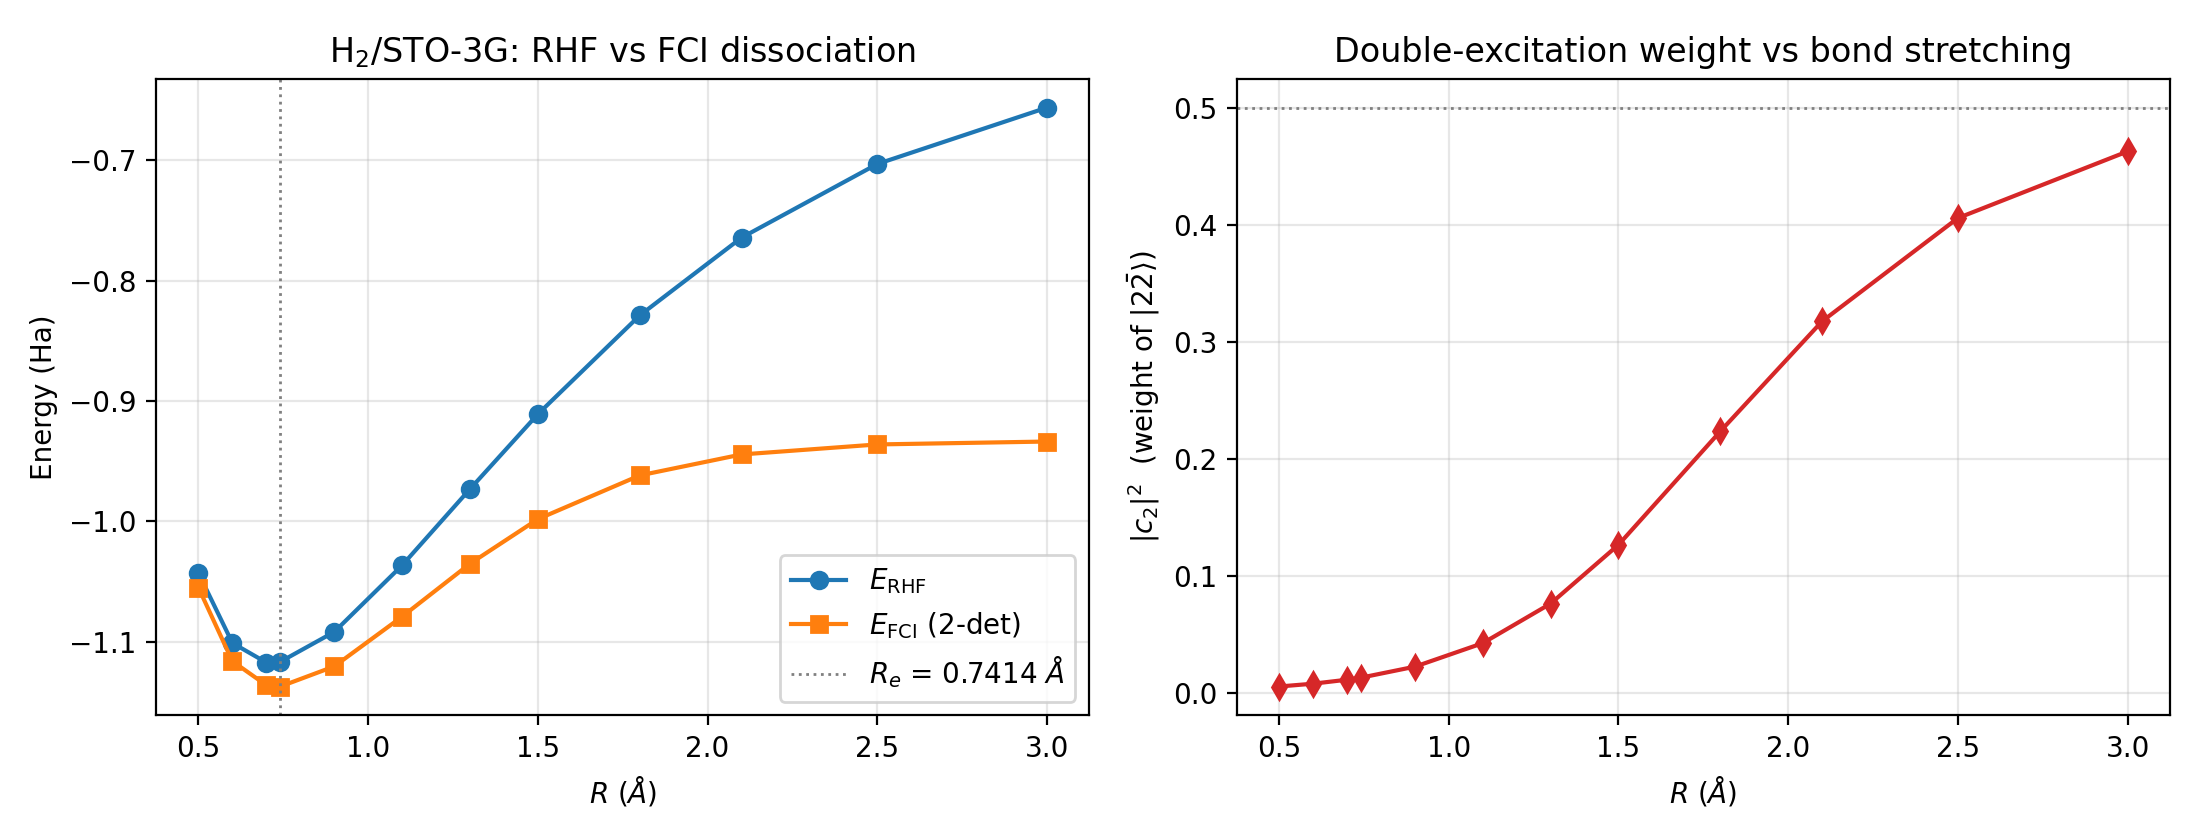
\includegraphics[width=\textwidth]{problem1_stretch.png}
\caption{Left: RHF vs two-determinant FCI dissociation curves of H$_2$/STO-3G.
Right: weight of the doubly excited determinant in the FCI ground state.}
\label{fig:p1stretch}
\end{figure}

\begin{table}[H]
\centering\small
\begin{tabular}{rrrrr}
\toprule
$R$ (\AA) & $E_\mathrm{RHF}$ (Ha) & $E_\mathrm{FCI}$ (Ha) & $E_\mathrm{corr}$ (Ha) & $|c_2|^2$ \\
\midrule
0.5000 & -1.042996 & -1.055160 & -0.012164 & 0.0052 \\
0.6000 & -1.101128 & -1.116286 & -0.015158 & 0.0076 \\
0.7000 & -1.117349 & -1.136189 & -0.018840 & 0.0110 \\
0.7414 & -1.116684 & -1.137270 & -0.020586 & 0.0127 \\
0.9000 & -1.091914 & -1.120560 & -0.028646 & 0.0221 \\
1.1000 & -1.036539 & -1.079193 & -0.042654 & 0.0422 \\
1.3000 & -0.973111 & -1.035186 & -0.062076 & 0.0760 \\
1.5000 & -0.910874 & -0.998149 & -0.087276 & 0.1263 \\
1.8000 & -0.828848 & -0.961817 & -0.132969 & 0.2233 \\
2.1000 & -0.764178 & -0.944375 & -0.180197 & 0.3173 \\
2.5000 & -0.702944 & -0.936055 & -0.233111 & 0.4056 \\
3.0000 & -0.656048 & -0.933632 & -0.277584 & 0.4626 \\
\bottomrule
\end{tabular}
\caption{Bond-stretching scan of H$_2$/STO-3G (\texttt{problem1.py}).}
\end{table}


% =====================================================================
\section{Problem 2: Qubit Mappings}
% =====================================================================

\textbf{Conventions} (as required by the problem statement): for JW and BK we
use the \emph{interleaved} ordering, qubit $p\leftrightarrow$ mode
$p\in\{0,1,2,3\}=(\chi_1,\chi_2,\chi_3,\chi_4)$; Pauli strings are written in
ascending qubit index. The two-qubit parity mapping uses the \emph{blocked}
ordering (modes $0,1=\sigma_g\alpha,\sigma_u\alpha$; modes
$2,3=\sigma_g\beta,\sigma_u\beta$); after the parity encoding, qubit~1 stores
the $\alpha$-electron number parity and qubit~3 the total number parity. For
the neutral $N_\alpha=N_\beta=1$ sector these are fixed to the eigenvalues
$Z_1=(-1)^{N_\alpha}=-1$ and $Z_3=(-1)^{N_\alpha+N_\beta}=+1$, and qubits 1 and
3 are removed.

\subsection*{(a) Anticommutation relations and the number operator}

With $a^\dagger_p=\tfrac12\big(\prod_{q<p}Z_q\big)(X_p-iY_p)$ and
$a_p=\tfrac12\big(\prod_{q<p}Z_q\big)(X_p+iY_p)$, define
$\sigma^\pm_p=\tfrac12(X_p\pm iY_p)$, which obey
$\sigma^+_p\sigma^-_p+\sigma^-_p\sigma^+_p=I$ and
$(\sigma^\pm_p)^2=0$. For $p=q$ the $Z$ strings square to the identity and
\begin{equation}
\{a_p,a^\dagger_p\}=\sigma^+_p\sigma^-_p+\sigma^-_p\sigma^+_p=I .
\end{equation}
For $p<q$ the string of $a_q^{(\dagger)}$ contains $Z_p$, which
\emph{anticommutes} with $\sigma^\pm_p$; moving $Z_p$ through $\sigma^\pm_p$
generates a relative minus sign between the two orderings, so
$\{a_p,a^\dagger_q\}=\{a_p,a_q\}=\{a^\dagger_p,a^\dagger_q\}=0$. Together,
$\{a_p,a^\dagger_q\}=\delta_{pq}$, i.e.\ JW preserves the fermionic algebra.
\texttt{problem2.py} verifies all $4\times4$ mode pairs symbolically at the
Pauli-algebra level: maximum deviation $\PtwoAcrDev$.

\textbf{Number operator.} The $Z$ strings of $a^\dagger_p$ and $a_p$ cancel:
\begin{equation}
n_p=a^\dagger_p a_p=\sigma^-_p\sigma^+_p
 =\tfrac14\,(X_p-iY_p)(X_p+iY_p)
 =\tfrac14\,(2I-2Z_p)
 =\tfrac{I-Z_p}{2},
\end{equation}
verified numerically to $\PtwoNumDev$ for every mode.

\subsection*{(b) Generated Hamiltonians}

All three Hamiltonians are generated from the STO-3G integrals of Problem~3
($E_\mathrm{nuc}$ included in the identity coefficient). The JW Hamiltonian has
exactly the structure of Eq.~(10) of the assignment --- 1 identity, 4 single-$Z$,
6 $ZZ$ and 4 weight-4 terms with the sign pattern
$X_0Y_1Y_2X_3=Y_0X_1X_2Y_3=-X_0X_1Y_2Y_3=-Y_0Y_1X_2X_3$ (asserted in code), with
$b_{11}=\PtwoBeleven\Ha$, which is precisely
$\tfrac14\braket{12}{34}$, the double-excitation coupling of
Eq.~\eqref{eq:fciblock}.

\begin{table}[H]
\centering\small
\begin{tabular}{lrr}
\toprule
Pauli string & weight & coefficient (Ha) \\
\midrule
\texttt{I} & 0 & -0.09886398 \\
\texttt{Z0} & 1 & +0.17119775 \\
\texttt{Z1} & 1 & +0.17119775 \\
\texttt{Z2} & 1 & -0.22278593 \\
\texttt{Z3} & 1 & -0.22278593 \\
\texttt{Z0\,Z1} & 2 & +0.16862219 \\
\texttt{Z0\,Z2} & 2 & +0.12054482 \\
\texttt{Z0\,Z3} & 2 & +0.16586702 \\
\texttt{Z1\,Z2} & 2 & +0.16586702 \\
\texttt{Z1\,Z3} & 2 & +0.12054482 \\
\texttt{Z2\,Z3} & 2 & +0.17434844 \\
\texttt{X0\,X1\,Y2\,Y3} & 4 & -0.04532220 \\
\texttt{X0\,Y1\,Y2\,X3} & 4 & +0.04532220 \\
\texttt{Y0\,X1\,X2\,Y3} & 4 & +0.04532220 \\
\texttt{Y0\,Y1\,X2\,X3} & 4 & -0.04532220 \\
\bottomrule
\end{tabular}
\caption{Jordan--Wigner Hamiltonian (4 qubits, interleaved ordering; $E_\mathrm{nuc}$ in the identity term).}
\end{table}

\begin{table}[H]
\centering\small
\begin{tabular}{lrr}
\toprule
Pauli string & weight & coefficient (Ha) \\
\midrule
\texttt{I} & 0 & -0.09886398 \\
\texttt{Z0} & 1 & +0.17119775 \\
\texttt{Z1} & 1 & +0.16862219 \\
\texttt{Z2} & 1 & -0.22278593 \\
\texttt{Z0\,Z1} & 2 & +0.17119775 \\
\texttt{Z0\,Z2} & 2 & +0.12054482 \\
\texttt{Z1\,Z3} & 2 & +0.17434844 \\
\texttt{X0\,Z1\,X2} & 3 & +0.04532220 \\
\texttt{Y0\,Z1\,Y2} & 3 & +0.04532220 \\
\texttt{Z0\,Z1\,Z2} & 3 & +0.16586702 \\
\texttt{Z0\,Z2\,Z3} & 3 & +0.12054482 \\
\texttt{Z1\,Z2\,Z3} & 3 & -0.22278593 \\
\texttt{X0\,Z1\,X2\,Z3} & 4 & +0.04532220 \\
\texttt{Y0\,Z1\,Y2\,Z3} & 4 & +0.04532220 \\
\texttt{Z0\,Z1\,Z2\,Z3} & 4 & +0.16586702 \\
\bottomrule
\end{tabular}
\caption{Bravyi--Kitaev Hamiltonian (4 qubits, interleaved ordering).}
\end{table}

\begin{table}[H]
\centering\small
\begin{tabular}{lrr}
\toprule
Pauli string & weight & coefficient (Ha) \\
\midrule
\texttt{I} & 0 & -0.33995362 \\
\texttt{Z0} & 1 & +0.39398368 \\
\texttt{Z1} & 1 & -0.39398368 \\
\texttt{X0\,X1} & 2 & +0.18128881 \\
\texttt{Z0\,Z1} & 2 & -0.01123659 \\
\bottomrule
\end{tabular}
\caption{Two-qubit parity-tapered Hamiltonian (blocked ordering; removed qubits 1 and 3 with $Z_1=-1$, $Z_3=+1$).}
\end{table}


\subsection*{(c) Eigenvalues in the neutral sector}

The two fixed $\mathbb{Z}_2$ sectors are the $\alpha$- and $\beta$-electron
number parities (the latter equivalently expressed through the total parity);
for neutral H$_2$, $N_\alpha=N_\beta=1$ gives $Z_1=-1$, $Z_3=+1$ as stated
above. Sector spectra are extracted by (i) direct determinant-basis projection
for the fermionic Hamiltonian, (ii) a penalty construction
$H+\lambda(\hat N_\alpha-1)^2+\lambda(\hat N_\beta-1)^2$ for JW and BK (the
number operators mapped through the same transformation), and (iii) the full
$4\times4$ spectrum of the tapered two-qubit Hamiltonian, whose Hilbert space
\emph{is} the neutral sector.

\begin{table}[H]
\centering\small
\begin{tabular}{crrrr}
\toprule
\# & fermionic & JW & BK & parity-tapered \\
\midrule
0 & -1.13727017 & -1.13727017 & -1.13727017 & -1.13727017 \\
1 & -0.53247901 & -0.53247901 & -0.53247901 & -0.53247901 \\
2 & -0.16990140 & -0.16990140 & -0.16990140 & -0.16990140 \\
3 & +0.47983610 & +0.47983610 & +0.47983610 & +0.47983610 \\
\bottomrule
\end{tabular}
\caption{The four eigenvalues (Ha) of the neutral $N_\alpha{=}N_\beta{=}1$ sector across representations.}
\end{table}


All four representations agree to $\PtwoSectorDev$, and the ground state
reproduces the benchmark $E_\mathrm{FCI}=-1.13727\Ha$ to $\PtwoFciErr$.

\subsection*{(d) Mapping comparison}

\begin{table}[H]
\centering\small
\begin{tabular}{lccc}
\toprule
mapping & qubits & non-identity terms & max Pauli weight \\
\midrule
JW & 4 & 14 & 4 \\
BK & 4 & 14 & 4 \\
parity-tapered & 2 & 4 & 2 \\
\bottomrule
\end{tabular}
\caption{Mapping comparison for minimal-basis H$_2$.}
\end{table}


For this 4-mode problem BK offers no term-count advantage over JW (both have 14
non-identity terms, maximum weight 4); its asymptotic
$\mathcal O(\log n)$-weight advantage only materializes for larger systems. The
parity mapping combined with $\mathbb{Z}_2$ tapering is strictly superior here:
2 qubits, 4 non-identity terms, maximum weight 2.

% =====================================================================
\section{Problem 3: Integrals and Ansatz Circuits}
% =====================================================================

\subsection*{(a) Integrals}

Computed with PennyLane \PLVersion\ (differentiable canonical RHF, STO-3G,
$R=0.7414$\,\AA). Integral convention: physicists' $\braket{pq}{rs}$ as in
Problem~1; the engine output is converted to chemists' order first and then to
physicists' order via $\braket{pq}{rs}=(pr|qs)$. One-based orbital labels
$1=\sigma_g$, $2=\sigma_u$:

\begin{table}[H]
\centering\small
\begin{tabular}{lrl}
\toprule
quantity & value (Ha) & chemists' \\
\midrule
$E_\mathrm{nuc}$ & +0.71375399 & \\
$h_{11}$ & -1.25246357 & \\
$h_{12}=h_{21}$ & -0.00000000 & (symmetry) \\
$h_{22}$ & -0.47594872 & \\
$\langle 11\vert 11\rangle$ & +0.67448877 & $= (11|11)$ \\
$\langle 11\vert 12\rangle$ & +0.00000000 & $= (11|12)$ \\
$\langle 11\vert 22\rangle$ & +0.18128881 & $= (12|12)$ \\
$\langle 12\vert 12\rangle$ & +0.66346810 & $= (11|22)$ \\
$\langle 12\vert 22\rangle$ & +0.00000000 & $= (12|22)$ \\
$\langle 22\vert 22\rangle$ & +0.69739376 & $= (22|22)$ \\
\bottomrule
\end{tabular}
\caption{RHF/STO-3G integrals of H$_2$ at $R=0.7414$\,\AA\ (physicists' notation; chemists' equivalent in the last column).}
\end{table}


The 8-fold permutation symmetry of Eq.~(16) holds to $\PthreePermDev$, and
integrals with an odd number of $\sigma_u$ factors vanish by $g/u$ parity, as
asserted in code. The RHF energy recomputed from these integrals,
$E_\mathrm{RHF}=\ErhfHtwo\Ha$, matches the assignment reference.

\subsection*{(b) Mapped Hamiltonians and exact diagonalization}

The JW, BK and parity-tapered Hamiltonians constructed from these integrals
(Tables in Problem~2) give identical neutral-sector ground-state energies,
\begin{equation}
E_0^{\mathrm{JW}}=E_0^{\mathrm{BK}}=E_0^{\mathrm{parity}}
=\EfciHtwoLong\Ha
\end{equation}
(mutual deviation $\le\PtwoSectorDev$), reproducing the FCI benchmark.

\subsection*{(c) UCCSD ansatz}

The UCC ansatz is $\ket{\psi(\theta)}=e^{\hat T-\hat T^\dagger}\ket{\mathrm{HF}}$.
For minimal-basis H$_2$, Brillouin's theorem plus $g/u$ symmetry remove all
single excitations (verified numerically:
$\max\lvert\bra{\mathrm{HF}}[H,\hat G_\mathrm{single}]\ket{\mathrm{HF}}\rvert=\PthreeBrillouin$),
leaving the single essential double amplitude
\begin{equation}
\hat T-\hat T^\dagger
=\theta\,\big(a^\dagger_2 a^\dagger_3 a_1 a_0 - a^\dagger_0 a^\dagger_1 a_3 a_2\big).
\end{equation}
Under JW this maps to eight mutually commuting weight-4 Pauli strings with
coefficients $\pm\theta/8$,
\begin{align}
e^{\hat T-\hat T^\dagger} = \exp\Big[-\tfrac{i\theta}{8}\big(
 &X_0X_1X_2Y_3+X_0X_1Y_2X_3-X_0Y_1X_2X_3-Y_0X_1X_2X_3 \nonumber\\
 +\,&X_0Y_1Y_2Y_3+Y_0X_1Y_2Y_3-Y_0Y_1X_2Y_3-Y_0Y_1Y_2X_3 \big)\Big],
\end{align}
so a \emph{first-order Trotter step is exact}: the circuit is the product of
eight standard Pauli-evolution blocks (basis change to $X/Y$, CNOT ladder,
$R_z(\pm\theta/4)$, undo), preceded by the HF preparation
$X_0X_1\ket{0000}=\ket{1100}$. Under the two-qubit parity-tapered mapping the
same generator collapses to
\begin{equation}
\hat T-\hat T^\dagger \;\longrightarrow\;
 -\tfrac{i\theta}{2}\,\big( X_0Y_1 - Y_0X_1 \big),
\end{equation}
a single-parameter two-qubit rotation, prepared on the tapered HF state
$\ket{01}=X_0\ket{00}$. Both circuits are drawn in
Figs.~\ref{fig:uccjw}--\ref{fig:uccpar}. Scanning $\theta$ on a statevector
gives $E(\theta^*)=\EfciHtwoLong\Ha$ at $\theta^*=\PthreeThetaOpt$ for both
mappings (error vs.\ FCI $<10^{-15}\Ha$), and $E(0)=E_\mathrm{RHF}$ as
required. Transpiled two-qubit gate cost: \PthreeCxJw\ CNOTs (JW) vs.\
\PthreeCxPar\ CNOTs (parity).

\begin{figure}[H]
\centering
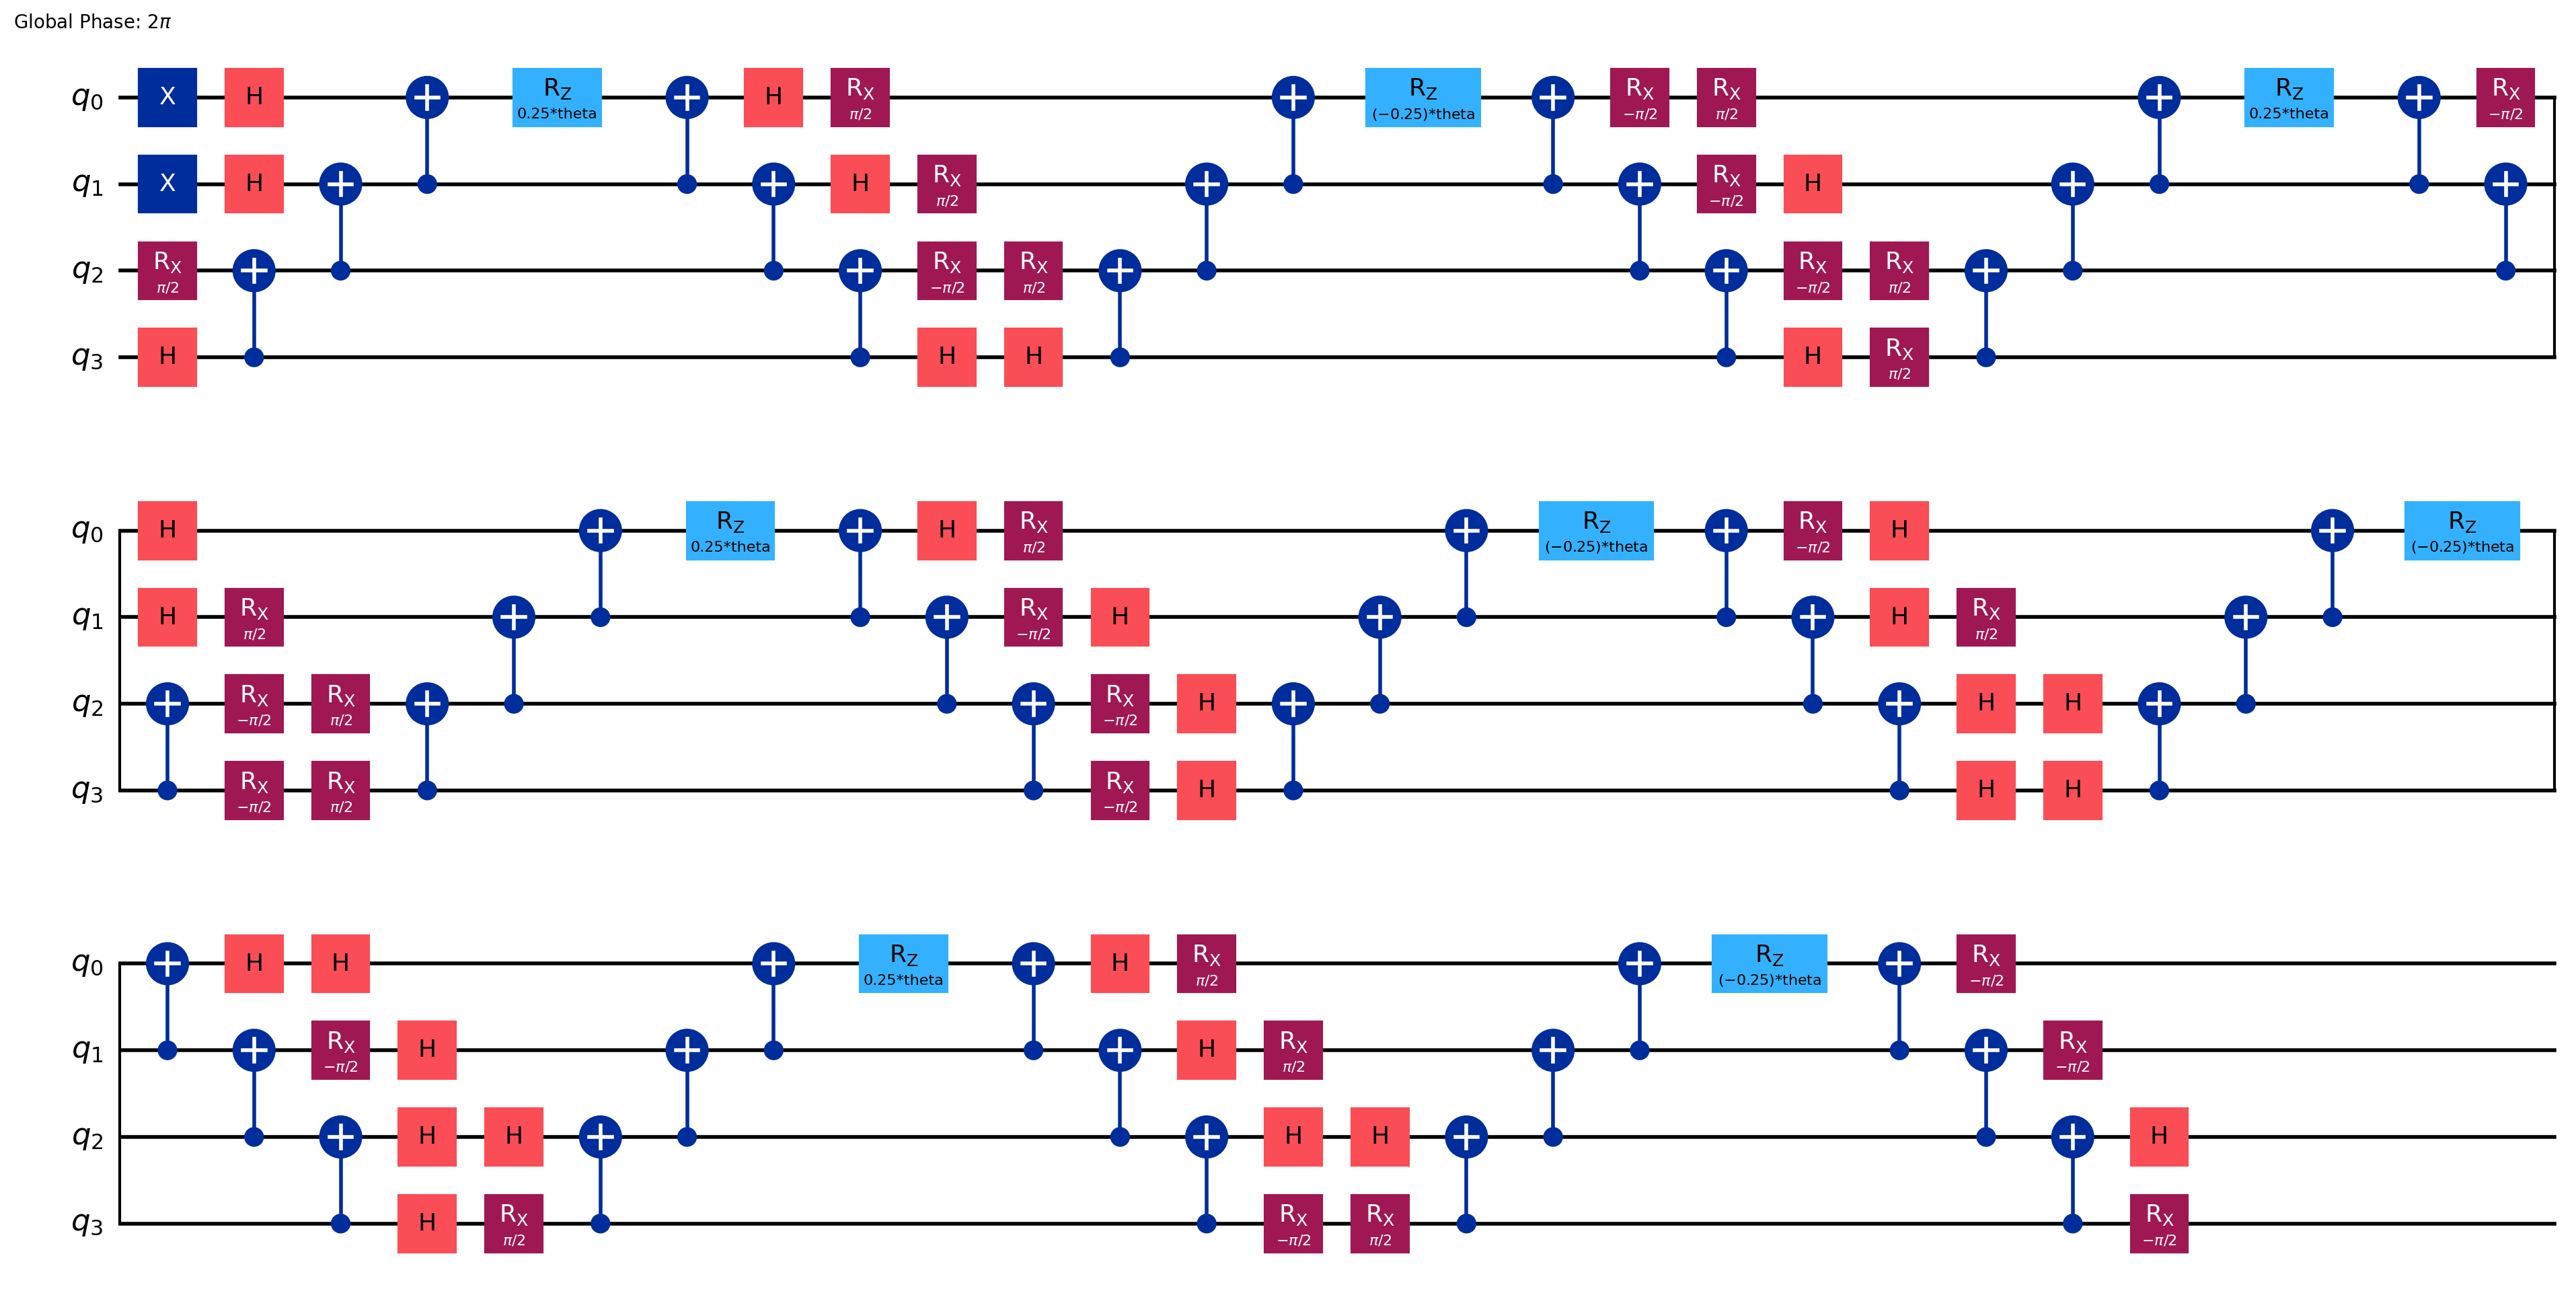
\includegraphics[width=\textwidth]{problem3_uccsd_jw.png}
\caption{UCCSD circuit, JW mapping (4 qubits): HF preparation $X_0X_1$ followed
by the eight exactly-Trotterized Pauli evolutions of the double-excitation
generator ($R_z$ angles $\pm\theta/4$).}
\label{fig:uccjw}
\end{figure}

\begin{figure}[H]
\centering
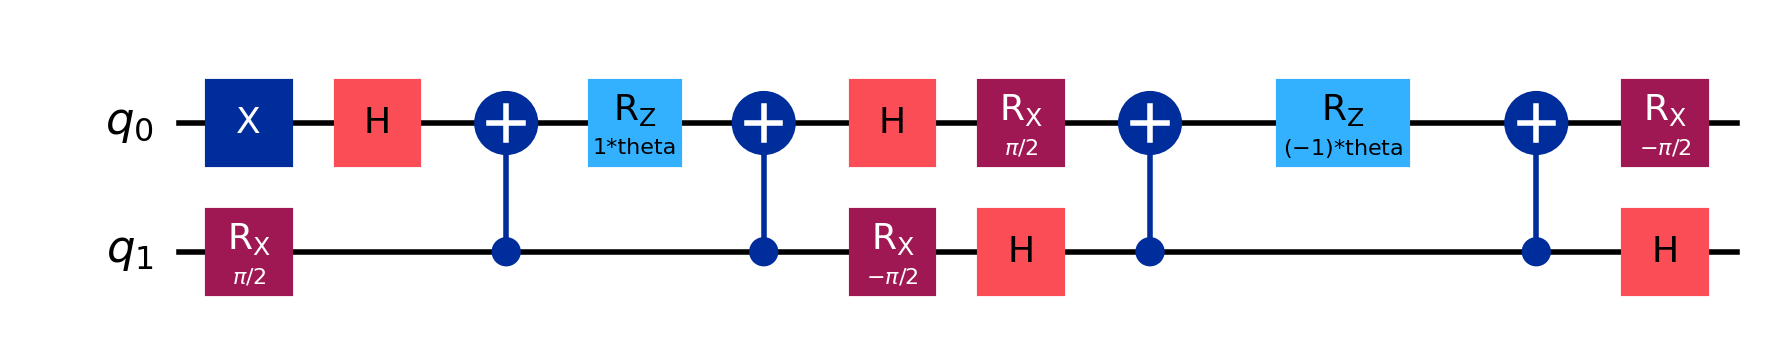
\includegraphics[width=0.85\textwidth]{problem3_uccsd_parity.png}
\caption{UCCSD circuit, two-qubit parity-tapered mapping: tapered HF
preparation $X_0$ and the single-parameter rotation
$\exp[-i\tfrac{\theta}{2}(X_0Y_1-Y_0X_1)]$.}
\label{fig:uccpar}
\end{figure}

\subsection*{(d) Real-amplitude hardware-efficient ansatz}

\begin{table}[H]
\centering\small
\begin{tabular}{lll}
\toprule
 & JW (4 qubits) & parity-tapered (2 qubits)\\
\midrule
initial state & $\ket{1100}=X_{q_0}X_{q_1}\ket{0}^{\otimes4}$ (HF) & $\ket{01}=X_{q_0}\ket{00}$ (tapered HF)\\
rotation gates & $R_y$ (real amplitudes) & $R_y$\\
entangler topology & linear CNOT chain $q_0\!-\!q_1\!-\!q_2\!-\!q_3$ (3 CX/layer) & single CNOT $q_0\!\to\!q_1$ per layer\\
layers / final rotations & 2 / yes & 2 / yes\\
parameters & 12 & 6\\
\bottomrule
\end{tabular}
\caption{Real-amplitude hardware-efficient ansatz specifications.}
\end{table}

\begin{figure}[H]
\centering
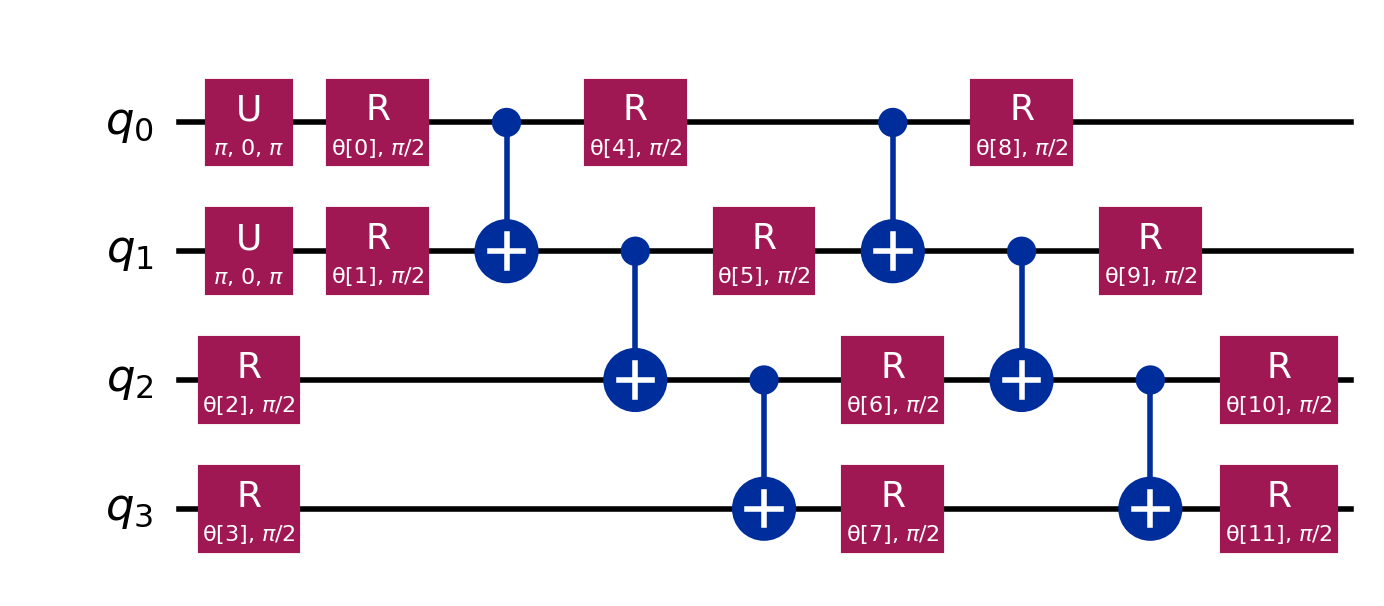
\includegraphics[width=0.95\textwidth]{problem3_hea_jw.png}
\caption{Real-amplitude ansatz, JW mapping (the leading $U(\pi,0,\pi)$ gates
are the HF preparation $X$ gates; $R(\theta_i,\pi/2)\equiv R_y(\theta_i)$).}
\end{figure}

\begin{figure}[H]
\centering
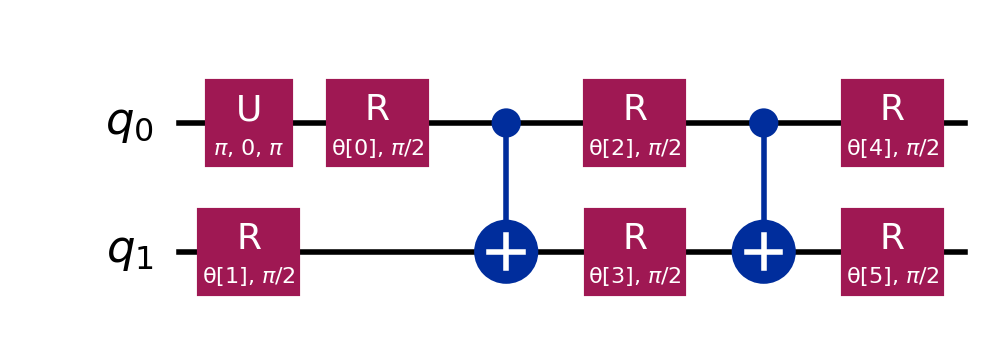
\includegraphics[width=0.6\textwidth]{problem3_hea_parity.png}
\caption{Real-amplitude ansatz, two-qubit parity-tapered mapping.}
\end{figure}

% =====================================================================
\section{Problem 4: VQE}
% =====================================================================

\subsection*{(a)+(b) Four noiseless VQE runs}

\textbf{Shared settings (stated once):} optimizer
\texttt{scipy} L-BFGS-B with numerical gradients, tolerance
$\mathtt{ftol}=10^{-10}$, $\mathtt{maxiter}=200$, initialization
$\theta_0\sim\mathcal N(0,0.1^2)$ drawn from
\texttt{numpy.random.default\_rng(13705049)} (re-seeded identically for every
case), simulator = exact statevector
(\texttt{qiskit.quantum\_info.Statevector}). The exact-diagonalization
reference of the same Hamiltonian is $\EfciHtwoLong\Ha$ for both mappings.

\begin{table}[H]
\centering\small
\begin{tabular}{lrrrcc}
\toprule
case & $E_\mathrm{VQE}$ (Ha) & $E_\mathrm{exact}$ (Ha) & abs.\ error & \#params & \#evals \\
\midrule
UCCSD+JW & -1.13727017 & -1.13727017 & \ensuremath{1.0\times10^{-16}} & 1 & 10 \\
UCCSD+parity & -1.13727017 & -1.13727017 & \ensuremath{4.4\times10^{-16}} & 1 & 10 \\
real-amplitude+JW & -1.13727017 & -1.13727017 & \ensuremath{2.2\times10^{-10}} & 12 & 572 \\
real-amplitude+parity & -1.13727017 & -1.13727017 & \ensuremath{4.8\times10^{-13}} & 6 & 49 \\
\bottomrule
\end{tabular}
\caption{VQE results on the noiseless statevector simulator (shared settings in the text).}
\end{table}


\begin{table}[H]
\centering\small
\begin{tabular}{l>{\raggedright\arraybackslash}p{10.5cm}}
\toprule
case & parameters \\
\midrule
UCCSD+JW & \texttt{-0.1131} \\
UCCSD+parity & \texttt{-0.1131} \\
real-amplitude+JW & \texttt{-20.4025, -31.6404, +24.7958, -10.9956, -4.7163, +10.7635, +58.0699, -4.7124, +7.6236, -1.9081, -25.1328, +15.7080} \\
real-amplitude+parity & \texttt{+0.0255, -0.1294, +0.2291, -0.1172, -0.0225, +0.0126} \\
\bottomrule
\end{tabular}
\caption{Optimized variational parameters.}
\end{table}


Both UCCSD circuits converge to the FCI energy at machine precision with only
10 objective evaluations (one well-conditioned parameter). The
hardware-efficient circuits also reach FCI, but the 12-parameter JW variant
needs $\sim$57$\times$ more evaluations --- a direct illustration of the value
of a physically motivated ansatz.

\subsection*{(c) Finite-shot estimation}

The best parity-tapered circuit (UCCSD+parity) is frozen at its noiseless
optimum $\theta^*$ and \emph{not} re-optimized. The 5-term Hamiltonian is
partitioned into qubit-wise commuting groups
$\{I,Z_0,Z_1,Z_0Z_1\}$ ($Z$ basis) and $\{X_0X_1\}$ ($X$ basis).
The shot budgets are $10^1=10$ and $10^4=10{,}000$ total shots.
\textbf{Shot-allocation rule:} the total budget is split equally over the
groups (remainder to leading groups), e.g.\ $10\to 5+5$. For each group the
energy contribution per shot,
$Y=\sum_k c_k(-1)^{\mathrm{parity}_k(\text{bits})}$, is averaged over the raw
outcomes; its sample variance automatically contains all intra-group
covariances (Appendix~C requirement), and group standard errors add in
quadrature.

\textbf{Backends.} Ideal: \texttt{qiskit-aer} \texttt{AerSimulator}
(shot-based, noiseless). Noisy: \texttt{AerSimulator.from\_backend(FakeBrisbane)};
target QPU \textbf{ibm\_brisbane} (127-qubit Eagle~r3), noise model from the
\texttt{qiskit-ibm-runtime} fake-provider calibration snapshot with median
parameters: $T_1=\PfourTone\,\mu$s, $T_2=\PfourTtwo\,\mu$s,
1Q ($\sqrt X$) error $\PfourSxErr$, 2Q (ECR) error $\PfourEcrErr$,
readout error $\PfourRoErr$; physical qubits $[0,1]$,
\texttt{seed\_simulator}=13705049.

\begin{table}[H]
\centering\small
\begin{tabular}{lrrrr}
\toprule
backend & shots & sample mean (Ha) & std.\ error (Ha) & mean $-$ $E_\mathrm{ref}$ \\
\midrule
ideal & 101 & -1.127348 & 0.025594 & +0.009922 \\
ideal & 10000 & -1.136005 & 0.003593 & +0.001265 \\
noisy & 101 & -0.996861 & 0.052869 & +0.140409 \\
noisy & 10000 & -1.064755 & 0.004691 & +0.072515 \\
\bottomrule
\end{tabular}
\caption{Finite-shot energy estimates of the frozen UCCSD+parity circuit ($E_\mathrm{ref}=-1.13727017$\,Ha).}
\end{table}


The ideal estimator is unbiased and its standard error shrinks as
$1/\sqrt{N}$ (within 1\,SE of the statevector optimum for both budgets). The
noisy backend shows a systematic $+\PfourNoisyBias\Ha$ bias at $10^4$ shots:
depolarizing-type gate noise and readout errors push the state towards the
maximally mixed state, raising the energy. Increasing shots reduces only the
statistical error bar, not this noise floor --- error mitigation, not more
sampling, would be required.

% =====================================================================
\section{Problem 5: Sample-based Quantum Diagonalization on LiH}
% =====================================================================

\paragraph{Method statement.} We follow \textbf{QSCI} (Kanno et al.\ 2023) as
a custom OpenFermion+NumPy build (explicitly allowed by the problem). Sampling
is noiseless, and the UCCSD state conserves particle number exactly, so
\textbf{no configuration recovery is applied} --- the measured probability
weight in the $(N_\alpha,N_\beta)=(2,2)$ sector is
$\PfiveSectorProb$.

\paragraph{System and reference values.} LiH/STO-3G at $R=1.5957$\,\AA, all 4
electrons in all 6 spatial orbitals = 12 spin orbitals = 12 qubits (JW,
interleaved). Computed: $E_\mathrm{nuc}=\PfiveEnuc\Ha$,
$E_\mathrm{HF}=\ErhfLih\Ha$, $E_\mathrm{FCI}=\EfciLihLong\Ha$ (sector exact
diagonalization) --- all matching the assignment references.

\paragraph{State preparation (amplitude source stated).} UCCSD with amplitudes
from \textbf{classical CCSD}: since PySCF is unavailable on native Windows, a
spin-orbital CCSD solver (Stanton et al.\ JCP \textbf{94}, 4334 (1991)
equations) was implemented in NumPy and converges in \PfiveCcsdIter\
iterations to $E_\mathrm{CCSD}=\PfiveEccsd\Ha$, matching the benchmark
$-7.88238\Ha$ to $\PfiveCcsdErr\Ha$ --- this benchmark validates the
implementation. The UCCSD state $e^{\hat T-\hat T^\dagger}\ket{\mathrm{HF}}$ is
applied exactly on the statevector (zero-Trotter-error reference of the UCCSD
circuit); its energy is $\PfiveEucc\Ha$, only
$\PfiveUccErr\Ha$ above FCI.

\paragraph{Bitstring/qubit ordering convention.} Qubit $p\leftrightarrow$ spin
orbital $p$ (interleaved: even $p$ = $\alpha$, odd $p$ = $\beta$ of spatial MO
$\lfloor p/2\rfloor$); OpenFermion basis index carries mode $p$ in bit
$(11-p)$; HF = modes $0..3$ occupied.

\paragraph{Sampling protocol.} A single stream of $10^5$ shots is drawn from
$\lvert\psi_x\rvert^2$ with \texttt{default\_rng(13705049)}; the budgets
$10^2,10^3,10^4,10^5$ are nested prefixes of this stream, so the CI subspaces
are nested and the energy converges monotonically (variational principle;
asserted in code). Bitstrings with occupations other than
$(2\alpha,2\beta)$ would be discarded; none occur (noiseless sampling).

\begin{table}[H]
\centering\small
\begin{tabular}{rrrrr}
\toprule
shots & $d$ & discarded & $E_\mathrm{SQD}$ (Ha) & $|E_\mathrm{SQD}-E_\mathrm{FCI}|$ \\
\midrule
$10^2$ & 3 & 0 & -7.87717099 & \ensuremath{5.2\times10^{-3}} \\
$10^3$ & 9 & 0 & -7.88214710 & \ensuremath{2.4\times10^{-4}} \\
$10^4$ & 10 & 0 & -7.88216883 & \ensuremath{2.2\times10^{-4}} \\
$10^5$ & 17 & 0 & -7.88230733 & \ensuremath{8.4\times10^{-5}} \\
\bottomrule
\end{tabular}
\caption{QSCI on LiH (4e,\,6o): unique kept determinants $d$, total energy and error vs.\ FCI for each shot budget (sector dimension 225).}
\end{table}


\begin{figure}[H]
\centering
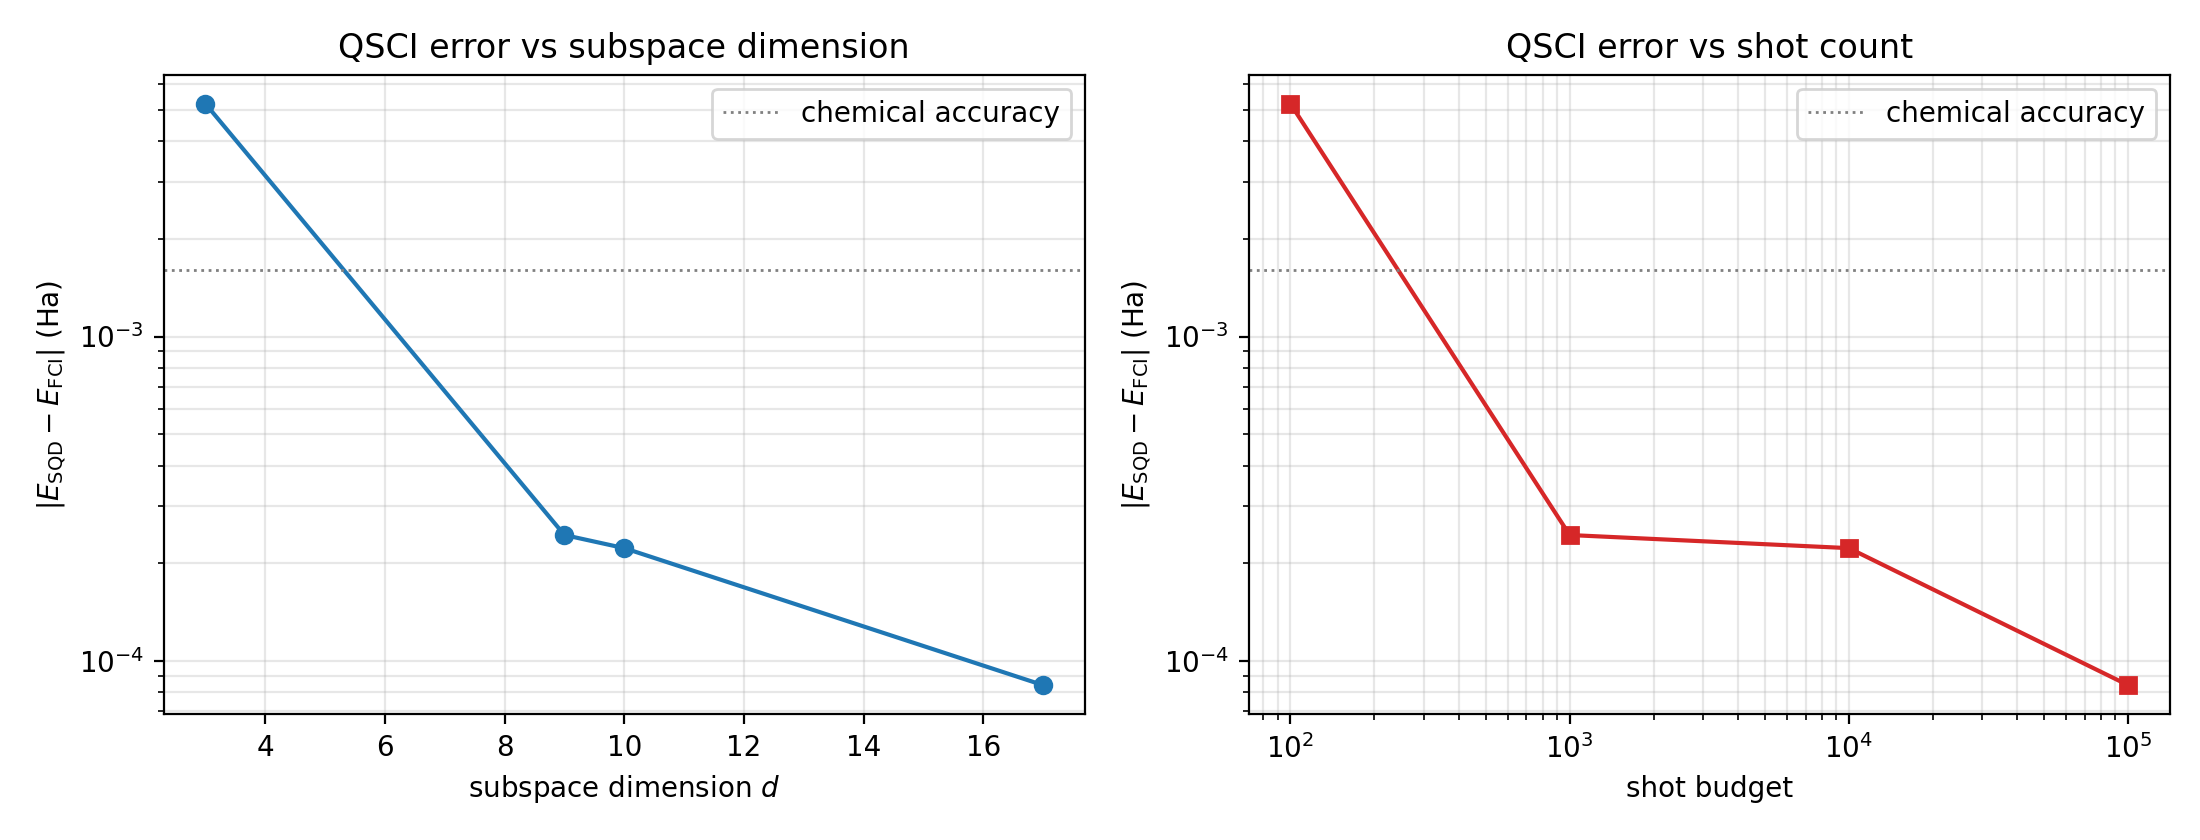
\includegraphics[width=\textwidth]{problem5_convergence.png}
\caption{QSCI convergence: $\lvert E_\mathrm{SQD}-E_\mathrm{FCI}\rvert$ versus
subspace dimension $d$ (left) and shot budget (right).}
\label{fig:p5conv}
\end{figure}

\paragraph{Scaling discussion.} The error drops below chemical accuracy
($1.6\,$mHa) already at $10^3$ shots with $d=9$ determinants out of the
$\binom{6}{2}^2=225$-dimensional sector --- the sampled subspace captures the
dominant correlation with a $\sim$4\% subspace fraction. Convergence then
proceeds in steps: a determinant enters the subspace only once its sampling
probability $\lvert c_x\rvert^2\gtrsim 1/N_\mathrm{shots}$, so each decade of
shots recruits the next tier of small-amplitude determinants
($\lvert c\rvert^2\sim10^{-5}\dots10^{-8}$ for LiH), giving the staircase
shape of Fig.~\ref{fig:p5conv} rather than a smooth power law. The ultimate
floor is set by how well the UCCSD distribution covers the FCI tail; at $10^5$
shots ($d=17$) the residual error is $\PfiveFinalErr\Ha$.

% =====================================================================
\appendix
\section{Code Availability}\label{app:code}
% =====================================================================

All scripts (\texttt{problem1.py}--\texttt{problem5.py},
\texttt{hw3\_common.py}, and \texttt{requirements.txt}) are available at
\url{https://github.com/crosses0612/QCAA-HW3}.

\end{document}
